
\chapter{Introduction}
\label{sec:intro}
We are in the era of autonomous driving: vehicles endowed with a wide variety of sensors, are becoming  capable to navigate in more and more challenging environments.
As humans,  autonomous vehicles exploit vision to perceive and interact with the surrounding environment.
Indeed, many advancements towards the autonomous driving have been achieved thanks to the joint efforts of Computer Vision and Robotics communities.

%Computer Vision aims at extracting meaningful information from images such as the class the subject belongs to, the action happening in the scene or the 3D model of the environment, while Robotics aims at designing robots, or autonomous machines, and at deploying them in the real world.

One of the key aspect in autonomous driving is the awareness of the surrounding provided by the map of the environment. 
To this regard, visual mapping and 3D reconstruction, represent two very active fields of research respectively in Robotics and in Computer Vision; both aim at modeling the scene captured through images.
Many works in Robotics focus on the real-time creation of the map while the camera is navigating through the environment, leading to the so called Visual Simultaneous Localization and Mapping (V-SLAM) algorithms. 
On the other hand, Computer Vision researchers tries to recover the  camera poses together with the structure of the map, in a batch fashion, with Structure from Motion (SfM) algorithms.
However, since the proposal of the Parallel Tracking and Mapping (PTAM) algorithm in \cite{klein_murray07} the methods adopted by the two communities became closer and closer, and eventually converged.

SfM and Visual SLAM algorithms build a point-based map of the environment that is often very sparse, except in the case of recent semi-dense SLAM, such as LSD-SLAM \cite{engel2014lsd}. 
Only few Dense-SLAM proposals, as DTAM \cite{newcombe2011dtam} or \cite{newcombe2010live}, are able to recover a dense representation of the scene, however they scales badly in large-scale environments, therefore they are not suitable for autonomous driving and urban scenes.

In Computer Vision, the evolution of the Structure from Motion algorithms are the  so called Multi-View Stereo (MVS) algorithms that recover a dense accurate reconstruction of the environment from a set of unordered images. 
MVS algorithms decouple the camera pose estimation and the model computation: they delegate the former task to an external algorithm, such as a SfM or a sensor fusion algorithm as \cite{mouragnon_et_al07} or \cite{cucci_matteucci13}, and they focus on the latter to estimate a detailed model of the environment.
As for the early SfM,  Multi-View Stereo focuses on accuracy but it has limited its application only to off-line  batch settings.


In the last decade, many Multi-View Stereo approaches have been proposed; they differ in various aspects, \eg, initialization, optimization procedure, 3D model representation, however the classical categorization \cite{seitz2006comparison} subdivides the algorithms according to the representation.
Depending on the approach, the scene can be represented by different geometric entities: points, 3D patches, volumes or surfaces.
Points are adopted when the available computational time is limited, \eg, in SLAM, and algorithms relying on 3D patches, which are small 3D portion of surfaces,  show impressive results on highly textured scenes as in \cite{furukawa2009reconstructing}. 
Since these two representation are designed to be sparse, they do not provide a continuous navigable surface, and they cannot be adopted for robot navigation.
%All the feature-based and semi-dense SLAM approaches, for computational reasons output such a sparse result, therefor their map are not suitable 

Nowadays, the Multi-View Stereo community turned to volumetric and mesh-based representations, that had got a boost thanks to the widespread availability of GPU hardware which enables massive parallel processing.
Volumetric algorithms partition the scene into voxels or tetrahedra and estimate a subset representing the free space and a subset representing the matter. The boundary between free space and matter represents the final 3D model of the scene (Figure \ref{fig:Volumetricc} illustrates an example in 2D). 

Mesh-based algorithms bootstrap from an initial mesh model of the scene and they evolve its shape in order to minimize the energy induced by the so called \emph{photometric error}.
Given a set of images and the corresponding 3D reconstruction, the photometric error specifies the likelihood of the reconstruction according to the images;  it is defined as the dissimilarity  between one image and the projection of a second image through the 3D model to the point of view of first image (see as Figure \ref{fig:reproj}).

Volumetric algorithms achieve very accurate results but their application is limited to small scene, since their data structure is not scalable. 
The best trade off between scalability and accuracy is achieved by the mesh-based algorithms which have been proven to score state of the art accuracy \cite{li2015detail} and to reconstruct large-scale scenes \cite{vu_et_al_2012}.


In mesh-based algorithms the initialization represents a crucial aspect.
A widespread initialization is known as visual hull, the reconstruction is the intersection of cones with the vertex in the camera and tangent to the perceived object.
Visual hull needs the knowledge of the silhouette of the objects, which is not a realistic assumption for real world scenarios.
Different approaches have been proposed to initialize the optimization, by relying on an intermediate volumetric approach, but the process requires human intervention to fix non manifold vertices, that induce inconsistencies in the mesh refinement.

\begin{figure}[tp]
 \centering
 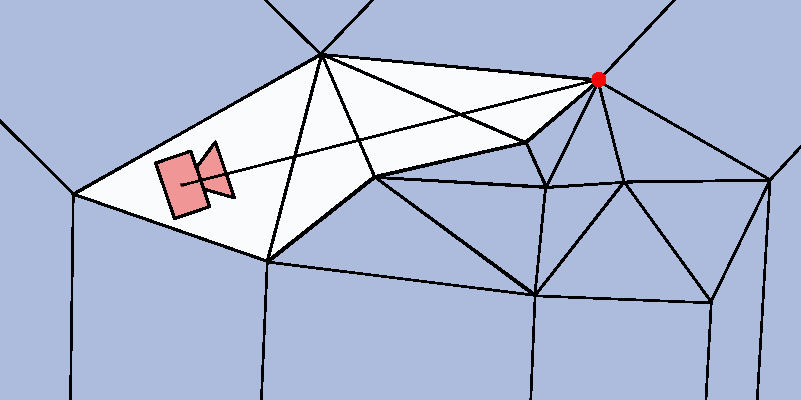
\includegraphics[width=0.85\columnwidth]{./img/spacecarv}
 \caption{Volumetric reconstruction: simple example on 2D case, dark triangles are matter white triangles are free space}
 \label{fig:Volumetricc}
\end{figure}


\section{Motivations}
To build a bridge between \mvs and dense SLAM we aim at preserving the positive aspects of the two approaches, dropping the drawbacks described thus far. 
On one side, the mapping algorithm has to manage large-scale outdoor environments, as in \mvs or non-dense SLAM approaches; at the same time it has to estimate an accurate model, comparable with the output of \mvs algorithms.
On the other  side, the algorithm has to estimate the map incrementally, as in SLAM algorithms.
An incremental algorithm allows to update an existing map with images that capture new regions of the environment, or with new images that add details about a part of the map already reconstructed.
%, as proved by Newcombe \etal \cite{newcombe2011dtam} or by Sch{\"o}ps \etal \cite{schops20153d}. 
For instance, a vehicle can capture new more detailed image about a reconstructed scene, or, during mapping campaigns or drone surveys, the operators could require to inspect the map while the images are  acquired in order to understand if more data have to be collected, \eg, where details are missing.


\begin{figure}[tp]
 \centering
 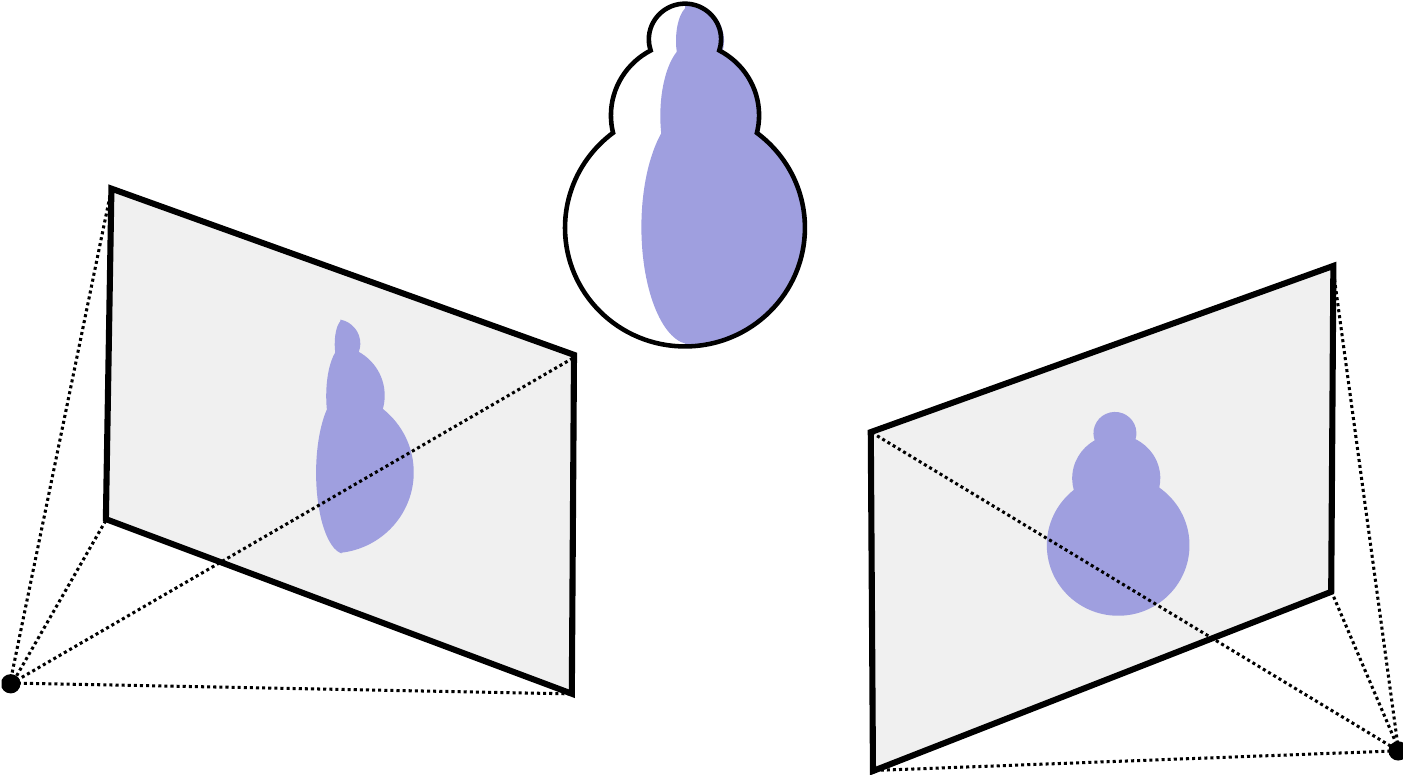
\includegraphics[width=0.925\columnwidth]{./img/reprojOr}
 \caption{Reprojection of image 2 on  image 1 through the model}
 \label{fig:reproj}
\end{figure}


The algorithms proposed in the literature are able to cover only part of these requirements.
Many works in \mvs focus on accurate small scale reconstruction; only recently mesh-based approaches have been able to combine scalability and accuracy. They are also able to represent the scene as  a continuous surface, which is very suitable for robotic applications, such as navigation.
However, state-of-the-art \mvs reconstruction pipelines are batch and not fully automatic. 
Classical SLAM provides an incremental estimation of the map, which is however very sparse.
Finally, dense SLAM algorithms are able to estimate incrementally a dense model, but it is limited to small indoor scenes or, in outdoor cases the output accuracy is not comparable to \mvs outputs and the reconstructed surface contains holes where the scene is untextured.

\section{Thesis contributions}
The key aspect of our proposal is to represent the scene as a triangular manifold mesh; the mesh representation allows us to reconstruct large-scale scenes though continuous meshes; the manifold property allows for coherent photometric mesh refinement. The building blocks of our pipeline are essentially two: incremental reconstruction from sparse points and incremental mesh refinement. The former step estimates a manifold mesh from the output of a Structure from Motion algorithm or any algorithm providing camera poses, sparse point clouds, and camera-to-point viewing rays (e.g., RGB-D and laser based systems). The latter step refines the resulting mesh according to the appearance provided by the images.

Our incremental reconstruction relies on a volumetric representation of the space based on the Delaunay triangulation; each tetrahedron of the triangulation is voted by the camera-to-point viewing rays crossing it and the manifold mesh is extracted as the boundary between those tetrahedra receiving high votes and those traversed by few or no rays. We investigated which kind of 3D points are suitable to build a Delaunay triangulation for 3D reconstruction, in particular in case of urban video sequences. Since 3D points on real-world edges usually project on points belonging to images edges, named  2D edge-points, we inverted this process by estimating the 3D position of 2D edge-points by tracking and triangulating them. When we build the triangulation upon reconstructed 3D edge-points, we bias the edges of tetrahedra connecting them to lay on real-world edges. This improves the representativeness of the triangulation and the accuracy of the reconstruction. We further improve our incremental algorithm with a novel voting scheme that generalizes state of the art results and improves the accuracy of the reconstruction; finally, we propose a simple, but effective, method to efficiently handle moving point inside the triangulation.

In low frequency sequences or in an unordered set of images where feature tracking fails, we noticed that a manifold mesh estimated from sparse data can sometimes be too far from the true 3D model of the scene. This would cause the subsequent mesh refinement process to get stuck in local minima or to converge slowly to the solution. Therefore, we improved the accuracy of the manifold mesh in order to speed up the refinement convergence and improve its the accuracy. To obtain this, we sweep the initial mesh in the space and we add to the point clouds the new 3D points for which the photometric matching score induced in a pair of camera is very high, which likely means that these points belong to the real scene.

Incremental mesh reconstruction, and mesh sweep refinement, output incrementally a low-resolution manifold mesh that feeds the refinement process of a novel incremental photometric refinement pipeline. Indeed, we proposed a novel approach to build an accurate map of the environment according to which, as a new partial mesh is reconstructed obtained, we evolve it photometrically and we merge it with an already refined mesh thanks to a novel merging algorithm which keeps the manifold property valid.

Aside from our pipeline, and motivated by the availability of lidar data often collected with images in autonomous driving applications, we tested and extended our mapping pipeline to work with hybrid lidar and image data. We proposed a complete mapping framework that leverages on the high accuracy of the 3D lidar data and on the appearance and density of images. By detecting and removing the moving points from lidar point clouds, we reconstruct the map of the scene with our reconstruction algorithm and we are able to refine it by neglecting the moving objects from the photometric optimization. Finally we recover a full textured map where moving points have been filtered out.

% \end{mdframed}
%\enlargethispage{2\baselineskip}
\section{Thesis outline}

The thesis is organized in three parts. 
In the first part we provide all the background materials needed to understand the contributions of the thesis.
\begin{itemize}
 \item Chapter \ref{ch:computational} gives an overview of the computational geometry tools we use in particular to describe how we reconstruct a manifold mesh.
 \item Chapter \ref{ch:camera} contains the classic definitions of pin-hole camera and the geometry behind the  multi-view setting, we also present how to formulate the pin-hole model in OpenGL, which adopts different conventions with respect the classical one.
\end{itemize}



% \begin{mdframed}[hidealllines=true,backgroundcolor=blue!20]

The second part of the thesis presents an overview on incremental reconstruction and it presents the main contributions of this thesis.
\begin{itemize}
 \item Chapter \ref{ch:soa} reviews the state of the art in mapping and Multi-View Stereo, focusing on the incremental reconstruction and on dichotomy between the Robotics and  Computer Vision algorithms propose to solve the same mapping problem from two different perspectives
 \item Chapter \ref{ch:manif} shows the incremental manifold reconstruction algorithm from a sparse point. We focus in particular on reconstruction from video sequences and we propose three contributions: a novel choice of the points adopted to build the volumetric representation of the scene through Delaunay Triangulation; a novel voting heuristic that prevents the creation of most artifacts in the mesh and a novel approach to manage moving points inside the triangulation.
 \item Chapter \ref{ch:sweeping} shows our mesh sweeping algorithm. In case of too sparse point clouds this algorithm adds new accurate 3D points to the reconstructed mesh, and it  improves the convergence and the accuracy of the refinement process.
 \item Chapter \ref{ch:incrDenseRef} illustrates the complete novel pipeline we propose to build incrementally a dense mesh on the environment; we focus in particular on the novel merging algorithm and on the refinement process.
\end{itemize}

In the third part of the thesis we illustrate our contribution aside from the incremental algorithm from image data:
\begin{itemize}
 \item Chapter \ref{ch:laser} presents our reconstruction approach extended to work with lidar data: we explicitly remove the moving point from the lidar point cloud and we leverage on the accurate 3D lidar estimate to build an accurate model of the environment, which we also refined and texturized through image data.
\end{itemize}

% \end{mdframed}
% In Chapter \ref{ch:further} we finally show some further experiments in which our algorithm plays a major role, in particular we show how the dense map can be adopted to localize a camera.




\section{Publications list}
We list the publications related to this thesis:
\begin{itemize}
 \item  A. Romanoni, M. Matteucci. Incremental reconstruction of urban environments by edge-points delaunay triangulation  \emph{IEEE / RSJ International Conference on Intelligent Robots and Systems (IROS), 2015} \cite{romanoni15b}.
 \item A. Romanoni, M. Matteucci. Efficient moving point handling for incremental 3D manifold reconstruction. \emph{International Conference on Image Analysis and Processing (ICIAP) 2015} \cite{romanoni15a}.
 \item A. Romanoni, A. Delaunoy, M. Pollefeys, M. Matteucci. Automatic 3D Reconstruction of Manifold Meshes via Delaunay Triangulation and Mesh Sweeping. \emph{Winter Conference on Applications of Computer Vision (WACV) 2016}. Best Paper Award. \cite{romanoni16}
 \item G. Postica,A. Romanoni, M. Matteucci. Robust Moving Objects Detection in Lidar Data Exploiting Visual Cues. \emph{IEEE / RSJ International Conference on Intelligent Robots and Systems (IROS), 2016}  \cite{postica16}.
 %\item A. Romanoni, D. Fiorenti, M. Matteucci. Visual and Laser data Fusion for Mesh-based 3D Photoconsistent Urban Mapping. submitted to \emph{IEEE International Conference on Robotics and Automation (ICRA), 2017}.
\end{itemize}










